\documentclass[openright]{report}
\usepackage{amsmath, amsfonts, chronosys, enumitem}
\usepackage[english]{babel}
\usepackage[T1]{fontenc}
\usepackage[utf8]{inputenc}
\usepackage[a5paper,inner=2.5cm,outer=1.5cm,top=2.0cm,bottom=1.5cm,head=0.7cm,foot=0.7cm]{geometry}

\newcommand{\random}{\stackrel{\$}{\longleftarrow}}

\title{Handling Vinegar Variables to Shorten Rainbow Key Pairs}
\author{Gustavo Zambonin}
\date{June 2019}

% \instituicao[a]{Universidade Federal de Santa Catarina}
% \departamento[o]{Departamento de Informática e Estatística}
% \curso[o]{Programa de Pós-Graduação em Ciência da Computação}
% \documento[a]{{Dissertação de Mestrado}}
% \titulo{Handling Vinegar Variables to Shorten Rainbow Key Pairs}
% \autor{Gustavo Zambonin}
% \grau{Mestre em Ciência da Computação}
% \local{Florianópolis}
% \data{12}{junho}{2019}
% \orientador[Orientador]{Ricardo Felipe Custódio, Dr.}

\begin{document}

\maketitle

\chapter{Introduction}

Handwritten signatures are one of the ubiquitous ways to ensure trust, in the case that a contract is sealed between parties. However, they present various logistical and security shortcomings. For instance, individuals are advised to be physically present to sign any documents, for they cannot be truthfully identified otherwise. Additionally, this kind of personal calligraphy can be forged with little effort. A solution coherent with the rise of the Information Age is found within mathematical frameworks known as signature schemes, that enable explicit assertions on the security of signatures.

A vibrant discipline of public-key cryptography, signature schemes are often associated with digital systems, in which transit of sensitive messages is expected to be secure. However, a specific scheme used within this situation drastically alters matters of security and performance compared to others. This is due to their natural connection to hard computational problems, that prevent forgery of signatures in various threat models. It is thus known that advances in computer engineering present direct consequences on the development of signature schemes.

Classical computers are electronic in nature, using circuits to perform computations. However, a new paradigm has emerged in the form of quantum computers, in which computations are performed outside the scope of classical mechanics. Although these computers are physically hard to implement, algorithms that make use of quantum phenomena have already been proposed and provably present a speedup compared to classical computers. One of these algorithms, due to Shor~\cite{Shor:199710:article}, simplifies the complexity of integer factorisation, and can be theoretically used to break widely used signature schemes.

Post-quantum cryptography addresses this issue by defining signature schemes which are either not known to be affected by quantum computers, or provably so~\cite{Bernstein:2008:book}. A popular technique employed to build quantum-resistant signatures is the usage of systems of equations over finite fields with multiple variables within the algorithms that rule the scheme. Primitives that use this strategy populate the area known as multivariate cryptography, and are extremely time- and space-efficient when creating and verifying signatures, while key generation is comparatively very slow and of large output.

Families of multivariate public-key cryptosystems are defined according to the types of finite fields used in the computations. This enables the focus on specific improvements, such as trade-offs between key and signature sizes, or larger security parameters. Particularly interesting are signature schemes based on the Oil--Vinegar principle, of which Rainbow~\cite{Ding:200506:inproc} receives primary attention. It performs computations on a single field and presents a balanced nature and simple, elegant definitions.

Large key sizes often impose constraints on the use of signature schemes in devices of limited storage and processing power. In multivariate cryptography, keys are often orders of magnitude larger than the ones used in conventional signature schemes. Due to this fact, several distinct approaches to reduce the key sizes of multivariate public-key cryptosystems have been proposed in the literature. In the case of Rainbow, to the best of our knowledge, these are distributed into methods that reduce exclusively private or public keys, but never both at the same time.

We address this fact by presenting a general framework that works for any Rainbow-like signature scheme, in which vinegar variables of the first layer are fixed in order to shorten the private key. This method allows for the use of techniques that reduce the public key on top of the existing modification, thus creating a Rainbow variant that has shorter private and public keys when compared to the classical scheme. We analyse the security implications of our proposal and show improvements with various parameter sets.

\section{Objectives}

We aim to create a novel method that enables the reduction of private and public key sizes in Rainbow-like signature schemes. Particularly, to support this goal, we wish to conduct a detailed study on the design of the Rainbow signature scheme and its variants. Further, the specific objectives are listed below:

\begin{enumerate}[label=(\roman*), itemsep=1pt]
  \item Classify strategies that enable compact representation of keys, \emph{e.g.} the use of particular data structures, algorithms or mathematical concepts;
  \item Establish the significance of structured private and public keys in the overall security of the schemes;
  \item Assess the consequences of shorter keys on the performance of the signature generation and verification steps;
  \item Produce a Rainbow-like signature scheme that can be combined with another chosen variant, allowing for the incorporation of benefits from both schemes.
\end{enumerate}

% TODO \section{Contributions of this thesis}

\section{Chronology}

We outline the dates for special occasions that lead altogether to the conclusion of a postgraduate qualification, namely a Master of Science degree, by the author. In no specific order, these consist of assorted activities related to the underlying program:

\begin{enumerate}[label=(\roman*), itemsep=1pt]
  \item\label{enum:0} defense of the studies conducted over the qualification period;
  \item\label{enum:1} writing a master's thesis;
  \item\label{enum:2} the acceptance of a scientific paper by an academic conference or journal;
  \item\label{enum:3} a minimum of credits from a given curriculum;
  \item\label{enum:4} a qualification exam;
  \item\label{enum:5} an English proficiency exam;
  \item\label{enum:6} attendance in events promoted by the program. 
\end{enumerate}

\begin{figure}[htbp]
  \vspace{-2cm}
  \begin{chronology}[startyear=2018, stopyear=2021, height=3pt, dates=false, arrow=false, align=center]
    \chronoperiodecoloralternation{lightgray, gray}
    \definechronoevent{sp}[textstyle=\footnotesize, 
      datesseparation=/, conversionmonth=false, year=false]
    \chronoperiode[dateselevation=5pt]{2018}{2019}{}
    \chronoperiode[dates=false]{2019}{2020}{}
    \chronoperiode[dateselevation=5pt]{2020}{2021}{}
    \chronosp[markdepth=-25pt, datestyle=\textbf]{30/07/2018}{\textbf{Start of M.Sc.}}
    \chronosp[markdepth=-60pt]{15/02/2019}{Exam~\ref{enum:5}}
    \chronosp[markdepth=55pt]{09/03/2019}{1\textsuperscript{st} submission~\ref{enum:2}}
    \chronosp[markdepth=5pt]{02/05/2019}{1\textsuperscript{st} notification~\ref{enum:2}}
    \chronosp[markdepth=-25pt]{12/06/2019}{Exam~\ref{enum:4}}
    \chronosp[markdepth=20pt]{20/01/2020}{2\textsuperscript{nd} submission~\ref{enum:2}}
    \chronosp[markdepth=-60pt]{20/03/2020}{2\textsuperscript{nd} notification~\ref{enum:2}}
    \chronosp[markdepth=-25pt]{01/06/2020}{Manuscript~\ref{enum:1}}
    \chronosp[markdepth=55pt]{01/07/2020}{Defense~\ref{enum:0}}
    \chronosp[markdepth=5pt, datestyle=\textbf]{30/07/2020}{\textbf{End of M.Sc.}}
  \end{chronology}
  \caption{Timeline for relevant events throughout the M.Sc. studies of the author, over the course of four semesters.}
  \label{fig:1}
\end{figure}

Most of these events are shown in Figure~\ref{fig:1}. We highlight at least two paper submissions to conferences, but only the most relevant dates are presented to prevent visual pollution. Furthermore, items~\ref{enum:3} and~\ref{enum:6} are to be completed until the execution of item~\ref{enum:4}, and are not pictured due to the high distribution of dates related to these activities. We expect that items~\ref{enum:2} to~\ref{enum:6} are finished within the first year of the degree, and the remaining items on the second year.

\section{Methodological approach}

In this section, we describe the research strategy applied to produce this work. Recall that the objects of study are the key sizes of Rainbow-like signature schemes. We define the main research question, parse the related body of literature, and finally apply several reproducible methods in order to infer conclusions. Indeed, this is essentially a description of the usual scientific method. In other words, we infer knowledge from mensurable experiments related to deductions, in the interest of solving specific limitations that come with the hypothesis.

\subsection{Literature review}\label{subsec:related}

We inspect formal works such as journal and conference articles, and monographs. We restrict ourselves to works published exactly after the first formal description of Rainbow~\cite{Ding:200506:inproc}, and particularly select ones that deal with reduction of key sizes. To conduct this analysis, the Google Scholar web tool was employed. It is a meta-indexer that covers most scientific literature providers, and allows the user to input advanced parameters in order to correctly narrow the needed scope.

The exact query used is \texttt{rainbow AND signature AND crypto AND (scheme OR post-quantum OR cryptography)}, searched over publications in English, no older than 2005, and not including patents. It is important to note that the keywords are searched over the entirety of the paper, whenever available. The query aims to reduce the amount of noise generated by the common name of the scheme, and as such, returns $\approx 1{,}150$ results. 

This is close to the number of works obtained when grouping all analogous searches in other sites, such as the ACM Digital Library, IEEE Xplore, Scopus, Semantic Scholar and Springer Link. Indeed, Google Scholar additionally crawls other sources, \emph{e.g.} university and governmental repositories, and as such returns a slightly larger number of works. From this set, we select relevant papers and present a summary below.

Schemes based on multivariate cryptography with modifications that enable the
reduction of private key sizes have been suggested even before Rainbow was
created. Tame transformation schemes, such as the ones listed
in~\cite{Wolf:200503:misc}, feature sparseness in their maps, a common
strategy used to shorten private keys, as seen in~\cite{Yang:200604:inproc}.
However, these schemes were either broken, as summarised
in~\cite{Ding:200604:article}, or in the case of Enhanced TTS, new parameters
were suggested, and it was subsequently found to be a special case of
Rainbow~\cite{Thomae:201207:inproc}.

Additionally, there are several published variations of Rainbow with the
same goal, making use of distinct approaches. A scheme called
Lite-Rainbow-0~\cite{Shim:201512:inproc} employs a small pseudorandom
number generator (PRNG) seed to replace the private key entirely. This shortens
the private key by a factor of approximately $99.8\%$, but greatly increases
the cost for signature generation. NC-Rainbow was proposed
in~\cite{Yasuda:201202:inproc}, with a novel strategy based in non-commutative
rings to reduce a private key by up to $75\%$. However, it was shown by
independent researchers to be
insecure~\cite{Thomae:201209:inproc,Hashimoto:201302:inproc}. Other variants
called MB-Rainbow~\cite{Yasuda:201305:inproc} and
NT-Rainbow~\cite{Yasuda:201404:inproc} employ sparseness of maps to reduce the
number of terms in the private key by up to $40\%$.

The authors merged MB- and NC-Rainbow into a single scheme called
MNT-Rainbow~\cite{Yasuda:201409:article}, shortening private keys by up to
$76\%$. Nevertheless, the original schemes were deemed insecure and new
parameters were suggested in~\cite{Peng:201706:article}. It also proposes a new
scheme called Circulant Rainbow, which reduces the private key by up to $45\%$
due to the concept of rotating relations. Yet, it was broken shortly
after~\cite{Hashimoto:201810:misc}. Furthermore, it appears that the introduction
of structures in the private key is highly threatening to the overall security 
of a Rainbow scheme.

In the case of modifications to the public key, there are mainly two approaches.
The approach by the authors of~\cite{Petzoldt:201006:inproc} is, to the best of 
our knowledge, the main method for public key reduction without compromises to
the signature size. It explores the fact that specific parts of the public key
do not contribute to the security of the scheme. It is summarised in several
publications~\cite{Petzoldt:201012:inproc,Petzoldt:201103:inproc,Petzoldt:201211:inproc,Petzoldt:201307:phd}
and used in~\cite{Shim:201512:inproc} to construct Lite-Rainbow-1.

The authors of~\cite{Szepieniec:201706:inproc} lift the public and central maps
of a particular case of Rainbow to an extension field, reducing its public 
key size by an order of magnitude but increasing the signature size. This is 
compatible with the generalised scheme, as seen in~\cite{Beullens:201706:msc,Beullens:201712:inproc},
and can make use of the improvements to the public key given above. However,
both of these strategies cannot be combined with the private key improvements
previously cited. 

\emph{Hypothesis.} It follows from the analysis above that, to the best of our knowledge, no works in the literature attempt to reduce both private and public keys in Rainbow-like signature schemes. This is due to the intricate relationship between both keys, in which one is used to create the other. Therefore, our hypothesis is answered positively if a scheme description is uncovered that shortens both keys in the key pair.

\subsection{Research method}

We enumerate below a chronological list of activities that depict the process used to develop our research.

\begin{enumerate}[label=(\roman*), itemsep=1pt]
    \item Maintain a bibliography featuring works related to reduction of keys in Rainbow-like signature schemes;
    \item Classify strategies used by scheme variants to reduce private or public keys;
    \item Develop a strategy to modify keys that is independent from existing ones;
    \item Test the scheme derived from this strategy against known cryptanalytic methods, particularly ones that take advantage of concepts used to devise this variant;
    \item Measure the overall gains of the scheme with regards to key sizes, comparing the new variant with existing works;
    \item Provide a reference implementation to show that our proposal does not deviate from default inputs and outputs.
\end{enumerate}

\chapter{Theoretical framework}

In this chapter, we will present the theory needed to understand how keys are reduced in Rainbow. In Section~\ref{sec:mult} a panorama of the discipline known as multivariate cryptography is given, with regards to the overall working and classification of schemes. A description of the Rainbow signature scheme is given in Section~\ref{sec:scheme}. 

% Finally, we give an overview of strategies used to reduce keys in Rainbow-like schemes in Section~\ref{sec:strat}.

\section{Multivariate cryptography}\label{sec:mult}

We will shortly present some basic mathematical definitions. Recall that a polynomial is a mathematical expression that consists of indeterminates, also called variables, and coefficients that multiply these variables. Only addition, subtraction, multiplication and integer exponentiation operations are permitted within polynomials. If we denote a $n$-uple of variables as $\mathbf{x} = (x_{1}, \dots, x_{n}), n \in \mathbb{N}$, a polynomial in this sequence is denoted $p(\mathbf{x})$. 

A polynomial may be separated into individual terms, called monomials. The degree of a monomial is the sum of the exponents of its variables, and the degree of a polynomial is the maximum degree between its monomials. A polynomial equation is constructed if we set $p(\mathbf{x}) = 0$. Finally, a polynomial system of $m \in \mathbb{N}$ equations is a set $\{p^{(1)}(\mathbf{x}) = 0, \dots, p^{(m)}(\mathbf{x}) = 0\}$ in which $\mathbf{x}$ is a common solution for all equations.

In some cases, polynomials have to be operated between themselves. Indeed, for a ring $R$, the set of all polynomials in $\mathbf{x}$ with coefficients from $R$ forms the polynomial ring $R[\mathbf{x}]$, where the additive and multiplicative identities are borrowed from $R$. With these concepts in mind, we can observe the classes of polynomials used within multivariate cryptography. Usually, cryptosystems are composed of systems of quadratic polynomials over finite fields, as pictured below:
\begin{align}
    \begin{split}
        \sum_{i = 1}^{n} \sum_{j = i}^{n} \alpha_{ij}^{(k)} x_{i} x_{j} + \sum_{i = 1}^{n} \beta_{i}^{(k)} x_{i} + \gamma_{0}^{(k)}, \\
        1 \leq k \leq m, \; \alpha, \beta, \gamma \in \mathbb{F}.
    \end{split}
\end{align}
The polynomial system above may also be represented as a mapping $\mathcal{M}: \mathbb{F}^{n} \to \mathbb{F}^{m}$.

This choice of degree is due to the fact that solving polynomial systems of non-linear nature is a proven NP-complete problem~\cite[Theorem 10]{Fraenkel:197909:article}. The simplest kinds of such systems are those composed of quadratic equations, indeed the most efficient in computations. Thus, they are widely used in multivariate cryptography.

% TODO origin of bipolar
We now turn to the main construction used in cryptosystems of multivariate nature. It is called bipolar, due to its elegant twofold nature. Consider $n, m \in \mathbb{N}$ as above. The function $\mathcal{M}: \mathbb{F}^{n} \to \mathbb{F}^{m}$ is generally called the central map, and it is regarded as the trapdoor, \emph{i.e.} a function that is easy to compute but difficult to invert without particular information. Two affine invertible maps $\mathcal{L}_{1} : \mathbb{F}^{n} \to \mathbb{F}^{n}$ and $\mathcal{L}_{2} : \mathbb{F}^{m} \to \mathbb{F}^{m}$ are used to hide the central map, by creating the composition $\mathcal{P} = \mathcal{L}_{1} \circ \mathcal{M} \circ \mathcal{L}_{2}$.

In terms of keys, it is evident that the private key is the $3$-uple $(\mathcal{L}_{1}, \mathcal{M}, \mathcal{L}_{2})$, whereas the public key is the map $\mathcal{P}$. With these definitions, it is possible to achieve both encryption and signature schemes, as seen in Figure~\ref{fig:2}. It depicts the steps used to operate on a message digest $h$. Particularly, if we look at the relation between $m$ and $n$, we conclude that if $m \geq n$, the application of the

\begin{figure}[htbp]
  \centering
  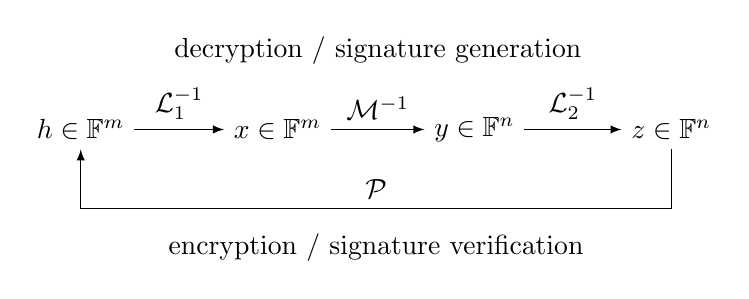
\begin{tikzpicture}
    \node (h) at (-2.5, 0) {$h \in \mathbb{F}^{m}$};
    \node (x) at (0, 0) {$x \in \mathbb{F}^{m}$};
    \node (y) at (2.5, 0) {$y \in \mathbb{F}^{n}$};
    \node (z) at (5, 0) {$z \in \mathbb{F}^{n}$};
    \draw[-latex] (h) -- (x) node[midway,above] {$\mathcal{L}_{1}^{-1}$};
    \draw[-latex] (x) -- (y) node[midway,above] {$\mathcal{M}^{-1}$}
      node[midway,yshift=1cm] {decryption / signature generation};
    \draw[-latex] (y) -- (z) node[midway,above] {$\mathcal{L}_{2}^{-1}$};
    \draw[-latex] (z) -- (5, -1) -- (-2.5, -1) node[midway,above]
      {$\mathcal{P}$} node[midway,yshift=-.5cm] {encryption / signature
      verification} -- (h);
  \end{tikzpicture}
  \caption{Standard flow of operations in the bipolar construction.}\label{fig:2}
\end{figure}

\section{Rainbow signature scheme}\label{sec:scheme}

We will present below a description of the Rainbow signature scheme, a
generalised version of Unbalanced Oil and Vinegar
(UOV)~\cite{Kipnis:199904:inproc}, that reduces the length of keys and
signatures. It consists of several ``oil and vinegar'' layers, that are
combined to create a ``rainbow''. Consider a finite field $\mathbb{F}_{q}$ and
$u, n \in \mathbb{N}$ where $u \leq n$. Choose a sequence of integers
$v_{1}, \dots, v_{u}$ such that
$0 = v_{0} < v_{1} < \cdots < v_{u} < v_{u + 1} = n$. Take the usual set
$V = \{1, \dots, n\}$ and define the vinegar variables as
$V_{l} = \{1, \dots, v_{l}\}$ for all $l \in \{1, \dots, u\}$. Observe that
$v_{l} = |V_{l}|$ and $V_{1} \subset \dots \subset V_{u} = V$. Oil variables
are given by $O_{l} = \{v_{l} + 1, \dots, v_{l + 1}\}$. Note that
$o_{l} = |O_{l}|$ and $O_{l} = V_{l + 1} - V_{l}$. Let $m = n - v_{1}$. Now,
we define vector spaces spanned by quadratic Oil-Vinegar polynomials of the
form
\begin{align}
  P_{l} = \sum_{i, j \in V_{l}} \alpha_{ij} \cdot x_{i} \cdot x_{j}
    + \sum_{i \in V_{l}, j \in O_{l}} \beta_{ij} \cdot x_{i} \cdot x_{j}
    + \sum_{i \in V_{l} \cup O_{l}} \gamma_{i} \cdot x_{i} + \delta.
\end{align}

\emph{Key generation.} The central map of Rainbow is defined as
$\mathcal{F} : \mathbb{F}^{n} \longrightarrow \mathbb{F}^{m}$, with the
following construction: for each layer $l$,
$F_{l} = (F_{l}^{1}, \dots, F_{l}^{o_{l}}) \random{} P_{l}$,
and $\mathcal{F} = (F_{1}, \dots, F_{l})$. Since each sequence of vinegar
variables in a layer contains all variables from the previous layer, this
allows for the inversion of this map. Further, let
$\mathcal{S} : \mathbb{F}^{m} \longrightarrow \mathbb{F}^{m}$ and
$\mathcal{T} : \mathbb{F}^{n} \longrightarrow \mathbb{F}^{n}$ be two affine
invertible maps, used as the trapdoor to this construction. Let
$\mathcal{P} : \mathbb{F}^{n} \longrightarrow \mathbb{F}^{m}$ as
$\mathcal{P} = \mathcal{S} \circ \mathcal{F} \circ \mathcal{T}$.
Coefficients $\alpha_{ij}, \beta_{ij}, \gamma_{i}, \delta \in \mathbb{F}$ are
chosen randomly. The private key is the triple
$(\mathcal{S}, \mathcal{F}, \mathcal{T})$ and the public key is the map
$\mathcal{P}$.

\emph{Signature generation.}
To sign a message $M$, consider a cryptographic hash function
$\mathcal{H} : {\{0, 1\}}^{*} \longrightarrow \mathbb{F}^{m}$, and obtain the
message digest $d = \mathcal{H}(M)$. The signature will be the set of variables
which yield the solution to the equation
$\mathcal{P}(x_{1}, \dots, x_{n}) = d$. Compute $x = \mathcal{S}^{-1}(d)$. To
generate $y = \mathcal{F}^{-1}(x)$, every layer must be inverted recursively.
Start by randomly choosing values for $x_{1}, \dots, x_{v_{1}}$ and inserting
them into the first layer. This will bring forth a system of $o_{1}$ linear
equations in $x_{v_{1} + 1}, \dots, x_{v_{2}}$. It can be solved with an
algorithm such as Gaussian elimination. If the system does not have a solution,
new vinegar variables have to be chosen. These solutions can then be
substituted into the next layer, which will create a system of $o_{2}$ linear
equations, that can be solved analogously. This procedure is repeated until all
layers are solved. Finally, we compute $\sigma = \mathcal{T}^{-1}(y)$.

\emph{Signature verification.}
To verify a signature, compute $d' = \mathcal{P}(\sigma)$. If $d = d'$, then
the signature is valid, and invalid otherwise.

Finally, denote an instance of the scheme by
Rainbow$(\mathbb{F}_{q}, v_{1}, o_{1}, \dots, o_{u})$. Note that when $u = 1$,
we get the UOV scheme. Measured in field elements, the size of a private key is
\begin{align}
  |\mathcal{K}_{Pr}| = m^{2} + m + n^{2} + n
    + \sum_{k = 1}^{u} o_{k} \cdot \left( \frac{v_{k} \cdot (v_{k} + 1)}{2}
      + v_{k} \cdot o_{k} + v_{k + 1} + 1 \right),
\end{align}
whereas the size of a public key is
\begin{align}
  |\mathcal{K}_{Pu}| = m \cdot \frac{(n + 1) \cdot (n + 2)}{2}.
\end{align}
Further details on the construction of Rainbow may be found
on~\cite[Section 3.3]{Ding:2006:book}.

% \section{Strategies to reduce keys}\label{sec:strat}

\chapter{Harnessing vinegar variables}

We will describe our improvement to Rainbow-like signature schemes below.
Sections~\ref{sec:mod} and~\ref{sec:efcma} give a formal description
of our modifications. In Section~\ref{sec:security}, we look into 
possible avenues of research to ensure that our proposal yields secure
schemes.

\section{Modification to the original scheme}\label{sec:mod}

Our approach consists of modifications to the key and signature generation
steps of Rainbow-like signature schemes. We propose to reuse the first set of
vinegar variables for several signatures and replace these only when necessary,
\emph{i.e.} situations where the central map cannot be inverted and creating a
signature would fail. By locking such variables and substituting them on the
central map $\mathcal{F}$ early in the key generation algorithm, we create a
$\mathcal{F}'$ linear in $v_{1}$, thus reducing storage requirements. This
approach does not modify the underlying structure of the private key, but
rather of the central map preimages.

To induce lower storage requirements for key pairs of Rainbow-like schemes, we
explore constructions given in the literature and suggest general alterations
to use our proposal. As per Subsection~\ref{subsec:related}, most variants that
shorten private keys are structural in nature, that is, the key space is
limited by some heuristic with the intent of producing a compact private key.
Moreover, the main approach to reduce public keys~\cite{Petzoldt:201307:phd}
prevents alterations to the private key,
since it indirectly generates $\mathcal{F}$ from a partial public key through
linear relations between the maps.

This division of improvements is blurred by our proposal. We present general
methods based on different techniques that shorten private keys in all
Rainbow-like schemes. We collectively denote these by Rainbow-$\eta$ and use
the same definitions as in Section~\ref{sec:scheme}, further denoting
the vinegar variables for the first layer as
$\widetilde{V}_{1} = (x_{1}, \dots, x_{v_{1}})$.

\emph{Rainbow-$\eta_{1}$ key generation.}
We use the fact that a PRNG has the ability to regenerate the same sequence of
numbers given a seed. The choice of such a generator is outside the scope of
our work, and we assume that a cryptographically secure PRNG is chosen. This
approach is similar to Lite-Rainbow-0, but it is not as costly, since the
private key does not need to be regenerated before every signature generation.
It is best suited to environments in which an efficient generator is previously
supplied.

We bound the creation of the key pair to a seed $\mathbf{S}$. We are not aware
of any Rainbow variants that disallow this practice. Thus, $\mathcal{S}$,
$\mathcal{F}$ and $\mathcal{T}$, as well as the public key
$\mathcal{P} = \mathcal{S} \circ \mathcal{F} \circ \mathcal{T}$ are generated
through the target scheme key generation algorithm, seeded by $\mathbf{S}$. We
set $\widetilde{V}_{1} \random{} \mathbb{F}$, and substitute these into
$\mathcal{F}$, giving $\mathcal{F}'$. In the rare case that a
failure occurs in the central map inversion algorithm, we use $\mathbf{S}$ to
regenerate $\mathcal{F}$, choose other values for $\widetilde{V}_{1}$ and
create a different $\mathcal{F}'$. The private key of Rainbow-$\eta_{1}$ is
$(\mathbf{S}, \mathcal{S}, \mathcal{F}', \mathcal{T})$ and the public key is
$\mathcal{P}$.

\emph{Rainbow-$\eta_{2}$ key generation.}
This approach is based on the fact that a private key owner is able to recover
the original $\mathcal{F}$ through the possession of all other private maps and
the public key. We make use of the linear relations given by the authors
of~\cite{Petzoldt:201006:inproc} and applied in the definition of the
well-known CyclicRainbow scheme. A short explanation is given below, with the
full rationale available in~\cite[Chapter 7]{Petzoldt:201307:phd}.

Consider the public key
$\mathcal{P} = \mathcal{S} \circ \mathcal{F} \circ \mathcal{T}$ and let
$\mathcal{Q} = \mathcal{F} \circ \mathcal{T}$. Denote $\widetilde{Q}$ as a
matrix containing only coefficients of the quadratic monomials from
$\mathcal{Q}$, and define $\widetilde{F}$ and $\widetilde{P}$ similarly.
Further let $\widetilde{T}$ be the matrix representation of $\mathcal{T}$, with
its coefficients $t_{ij}, i, j \in \{1, \dots, n\}$, and define $\widetilde{S}$
analogously. By fixing $t_{ij}$, the composition of $\mathcal{P}$ actually
represents a linear relation between coefficients $q_{ij}^{k}, f_{ij}^{k}$ of
the monomial $x_{i} \cdot x_{j}$ in the $k$-th component of, respectively,
$\mathcal{Q}$ and $\mathcal{F}$, with the form
\begin{align}
  \begin{split}
    q_{ij}^{k} = \sum_{r = 1}^{n} \sum_{s = r}^{n}
      \alpha_{ij}^{rs} \cdot f_{rs}^{k}, \quad
      \alpha_{ij}^{rs} = \begin{cases}
        t_{ri} \cdot t_{si}                         & \text{if } i = j, \\
        t_{ri} \cdot t_{sj} + t_{rj} \cdot t_{si}   & \text{otherwise},
      \end{cases} \\
      k \in \{v_{1} + 1, \dots, n\}.
  \end{split}
\end{align}
This can be simplified, since $\mathcal{F}$ does not allow quadratic monomials
with only oil variables, and results in
\begin{align}
  q_{ij}^{k} = \sum_{r = 1}^{v_{l}} \sum_{s = r}^{v_{l + 1}}
    \alpha_{ij}^{rs} \cdot f_{rs}^{k},
      \quad k \in O_{l}, \quad l \in \{1, \dots, u\}.
\end{align}
A square matrix of order $\frac{n^{2} + n}{2}$ is created to further streamline
the previous equations. Given a particular monomial ordering, let
$A = (\alpha_{ij}^{rs})$ such that $i, j, r, s \in \{1, \dots, n\}$, where
$i \leq j$ and $r \leq s$ denote row and column indices, respectively. Thus, we
have that $\widetilde{P} = \widetilde{S} \cdot \widetilde{Q}$ and
$\widetilde{Q} = \widetilde{F} \cdot A^{\text{T}}$. We note that the
performance of this method is lower than that of Rainbow-$\eta_{1}$. However,
it is a general technique that works on all Rainbow-like schemes.

Observe that the central map may not feature any linear or constant terms, due
to the use of the above relations. This does not lower the overall security of
the scheme, due to the fact that they are not multiplied with quadratic terms.
With this implication in mind, the usual key generation algorithm for the
target scheme is employed, yielding $(\mathcal{S}, \mathcal{F}, \mathcal{T})$
and $\mathcal{P}$ at a marginally faster rate. Substitute the sequence
$\widetilde{V}_{1} \random{} \mathbb{F}$ into $\mathcal{F}$, giving
$\mathcal{F'}$. By the relations above, one is able to reconstruct
$\mathcal{F}$ with no additional mechanisms if the central map inversion
algorithm fails. The private key of Rainbow-$\eta_{2}$ is
$(\mathcal{S}, \mathcal{F}', \mathcal{T})$ and the public key is $\mathcal{P}$.

\emph{Signature generation.}
A digest $d = \mathcal{H}(M)$ from a message $M$ is signed with a similar
procedure. Compute $x = \mathcal{S}^{-1}(d)$, and attempt to generate
$y = \mathcal{F}'^{-1}(x)$ by inverting every layer recursively. The first
layer already has $\widetilde{V}_{1}$ set, and the remaining linear system
needs only to be solved by providing appropriate values of $d$. It will
generate a new set of vinegar variables, that can be used on the next layer,
until all layers are solved. If any of the transitory systems are not solvable,
a new $\widetilde{V}_{1}$ is chosen and $\mathcal{F}'$ regenerated, according
to one of the methods given above. We finish by computing
$\sigma = \mathcal{T}^{-1}(y)$.

\emph{Signature verification.}
This step does not change. If $d = \mathcal{P}(\sigma)$, then the signature is
valid, and invalid otherwise.

By making the first layer linear and substituting the remaining variables, the
size of the private key is now
\begin{multline}
  |\mathcal{K}_{Pr}^{\eta}| = m^{2} + m + n^{2} + n
    + |\widetilde{V}_{1}| \\
    + \sum_{k = 1}^{u} o_{k} \cdot \left( \frac{(v_{k} - v_{1})(v_{k} - v_{1} + 1)}{2}
      + (v_{k} - v_{1}) \cdot o_{k} + (v_{k + 1} - v_{1}) + 1 \right),
\end{multline}
plus the additional size of $\mathbf{S}$ if the Rainbow-$\eta_{1}$ method is
used. One needs to store $\widetilde{V}_{1}$, since it is part of the central
map preimage, used on further map applications. The public key size does not
change.

\section{Application to the EF-CMA variant}\label{sec:efcma}

The Rainbow submission to the NIST standardisation
process~\cite{Ding:201712:misc} presents a scheme description that diverges
from the original works. The authors introduce modifications that provide
security against the existential forgery under chosen-message attack
model, whereas the original scheme only offers security against universal
forgery. These changes are built upon the introduction of a random salt. We
will briefly describe this approach, with the intent of preventing the
recalculation of $\mathcal{F}'$ in the case that $\widetilde{V}_{1}$ is not
suitable. Let us denote this method as \textbf{Rainbow-}$\mathbf{\eta_{3}}$.

\emph{Key generation.}
Consider $w \in \mathbb{N}$ as the length of the aforementioned salt. Generate
private and public keys as per Section~\ref{sec:scheme}. The private key
for this scheme is $(\mathcal{S}, \mathcal{F}', \mathcal{T}, w)$, with the
addition of $\mathbf{S}$ in the case of Rainbow-$\eta_{1}$. The public key is
$(\mathcal{P}, w)$.

\emph{Signature generation.}
Let $r \random{} {\{0, 1\}}^{w}$. The digest value is calculated as
$\mathbf{d} = \mathcal{H}(\mathcal{H}(M) \mid\mid r)$, where $M$ is the
message. The value $x = \mathcal{S}^{-1}(\mathbf{d})$ is obtained as usual. In
the rare case that the $y = \mathcal{F}'^{-1}(x)$ preimage calculation does not
succeed, new variables in $\widetilde{V}_{1}$ are chosen. However, the
addition of a random salt to the original message digest alters $\mathbf{d}$
completely, due to the cryptographic hash function application. Thus, it is
only necessary to generate a new $r$ and restart the signature generation
process, such that $\widetilde{V}_{1}$, and consequently $\mathcal{F}'$, are
not modified. Alternatively, if the preimage is generated successfully, we
finish by letting $z = \mathcal{T}^{-1}(y)$ and $\sigma = (z, r)$.

\emph{Signature verification.}
Recalculate the digest value $\mathbf{d}$. If $\mathbf{d} = \mathcal{P}(z)$,
the signature is valid, and invalid otherwise.

The size of the private and public keys increase in exactly one element due to
the addition of $w$.

\section{Security of our variants}\label{sec:security}

Recall that, to create a Rainbow signature, the central map $\mathcal{F}$ needs
to be inverted. Random guessing of vinegar variables is done in order to create
a solvable linear system. It is also known that the central map is expressed as
multivariate systems of equations, which can be themselves interpreted as
multidimensional matrices of coefficients. 
With this in mind, we propose to calculate the probability that a
random matrix with elements in $\mathbb{F}$ is invertible. This will prove useful
to conclude that the cost of recalculating $\mathcal{F}'$ is amortised over
multiple signatures.

Vinegar variables chosen to invert the central map are an integral part of the
preimage $y = \mathcal{F}^{-1}(x)$. 
Further, recall that there are approximately $q^v$ possibilities for $y$. Our
proposal eliminates this choice by locking vinegar variables into the private
key. Hence, it is essential to know if such variables create patterns in which
private information may leak through a multi-target attack. Experiments that
look for patterns in matrices and vectors with field elements from a
cryptographically secure pseudo-random number generator should aid in this objective.

Finally, a variety of attacks currently thwart the security of Rainbow-like
signature schemes if parameters are not chosen carefully. We will briefly
state each of those, along with their estimated complexities~\cite{Petzoldt:201005:inproc},
and argue that our methods do not facilitate such attacks.

\bibliographystyle{alpha}
\bibliography{ref}

\end{document}
